\documentclass{article}
\usepackage{icml2025}

\usepackage{microtype}
\usepackage{graphicx}
\usepackage{booktabs}
\usepackage{amsmath,amssymb,amsthm}
\usepackage{mathtools}
\usepackage{tikz}
\usetikzlibrary{positioning,trees,matrix}

\theoremstyle{plain}
\newtheorem{theorem}{Theorem}[section]
\newtheorem{lemma}[theorem]{Lemma}
\newtheorem{proposition}[theorem]{Proposition}
\newtheorem{corollary}[theorem]{Corollary}
\theoremstyle{definition}
\newtheorem{definition}[theorem]{Definition}
\theoremstyle{remark}
\newtheorem{remark}[theorem]{Remark}
\newtheorem{assumption}[theorem]{Assumption}

\icmltitlerunning{Short Title}

\begin{document}

\twocolumn[
\icmltitle{<Full Paper Title>}

\begin{icmlauthorlist}
\icmlauthor{First A. Author}{xxx}
\icmlauthor{Second B. Author}{yyy}
\icmlauthor{Third C. Author}{zzz}
\end{icmlauthorlist}

\icmlaffiliation{xxx}{Affiliation One, City, Country}
\icmlaffiliation{yyy}{Affiliation Two, City, Country}
\icmlaffiliation{zzz}{Affiliation Three, City, Country}

\icmlcorrespondingauthor{First A. Author}{first.last@institution.edu}

\icmlkeywords{Machine Learning, ICML}
\vskip 0.3in
]

\printAffiliationsAndNotice{}

\begin{abstract}
\end{abstract}

\section{Introduction}

\section{Related Work}

Structured reasoning with language models has become a prominent research direction. One foundational approach is \emph{Chain-of-Thought (CoT) prompting}, which elicits intermediate reasoning steps from the model. By having the model ``think aloud'' through a series of sub-steps, CoT significantly improves performance on complex tasks~\cite{wei2022chain}. Building on this idea, more advanced frameworks allow branching and search over possible reasoning paths instead of following a single linear chain. For example, \emph{Tree-of-Thoughts (ToT)} generalizes CoT by expanding a tree of potential ``thought'' steps and using self-evaluation to decide among branches, enabling lookahead and backtracking during inference~\cite{yao2023tree}. Such deliberate search over a reasoning tree or DAG can yield far better results on tasks requiring planning or strategic exploration, as the model is not confined to greedy left-to-right generation. Relatedly, alternative decoding strategies like self-consistency have been proposed to improve reliability: instead of taking one pass through the prompt, the model samples multiple diverse reasoning chains and then selects the most consistent answer among them~\cite{wang2022selfconsistency}. This method leverages the intuition that a complex problem may be solved via different logical routes leading to the same answer, and indeed has been shown to greatly boost accuracy on benchmarks~\cite{wang2022selfconsistency}.

Another line of work augments language model reasoning with \emph{external tools or formal executors}. \emph{Program-Aided Language Models (PAL)} exemplify this trend by generating programs (e.g., Python code) as intermediate reasoning steps and offloading their execution to a runtime~\cite{gao2023pal}. In PAL, the language model’s job is to correctly decompose the problem into code, and the Python interpreter handles the actual calculation or logic—an approach that achieved state-of-the-art results on math and symbolic reasoning tasks, even outperforming much larger models that rely on CoT alone~\cite{gao2023pal}. Beyond code execution, researchers have equipped LMs with a variety of \emph{tool-use abilities}. \emph{Toolformer} showed that an LM can be fine-tuned (in a self-supervised way) to decide when to call external APIs (such as calculators, web search, or translation services) and how to incorporate the results into its text generation~\cite{schick2023toolformer}. This allows the model to overcome its weaknesses (e.g., factual lookup, arithmetic) by delegating those subtasks to specialized tools, substantially improving zero-shot performance without sacrificing general language ability. In a similar vein, prompting strategies like \emph{ReAct} intermix textual reasoning with explicit actions. ReAct prompts the model to produce both \emph{Thoughts} (natural language reflections) and \emph{Actions} (commands like queries to a knowledge base or environment) in an interleaved manner~\cite{yao2023react}. By design, the model’s ``thought'' can trigger an external tool (e.g., a Wikipedia lookup) and then incorporate the tool’s output before continuing the reasoning. This tight integration of tool usage within the reasoning process helps address issues like hallucination and enables tackling interactive decision-making tasks that pure text generation would struggle with~\cite{yao2023react}. Overall, these tool-augmented systems demonstrate the benefit of extending LMs beyond the text-only paradigm—a theme also reflected in many recent agent frameworks.

Indeed, there has been a surge of interest in treating LMs as \emph{autonomous agents or planners} that can control their own multi-step decision process. Projects such as AutoGPT and BabyAGI (2023) popularized the idea of an ``AI agent'' that recursively plans and executes sub-goals using an LLM at its core~\cite{shen2023hugginggpt}. While these systems are outside traditional academic publications, they illustrate a trend of wrapping an LM in a loop of plan–act–observe, allowing it to tackle complex, long-horizon tasks. Academic work has explored similar ideas. For instance, \emph{Reflexion} proposes an LLM agent that improves itself through textual self-feedback: after each trial or attempted solution, the agent generates a natural-language reflection on what went wrong or could be improved, stores this in memory, and uses it to inform the next attempt~\cite{shinn2023reflexion}. Notably, this is done without gradient updates—the model refines its behavior by reading its own past reflections, a form of verbal self-reinforcement. This procedure led to large gains on tasks like code synthesis by enabling the agent to learn from mistakes in a few-shot manner~\cite{shinn2023reflexion}. Another example is \emph{HuggingGPT}, which treats a powerful LM (ChatGPT) as a high-level controller that can delegate subtasks to other specialized models. Given a complex request, HuggingGPT uses the LM to parse the task, generate a structured plan in natural language (identifying which models or tools to use for each subtask), call those models, and then integrate their outputs~\cite{shen2023hugginggpt}. Language serves as the interface between the controller LM and various tools or model ``friends,'' showcasing how an LM’s planning can orchestrate an entire tool ecosystem. Broadly, these approaches with learned or explicit controllers (ReAct, AutoGPT, Reflexion, etc.) share a motivation with NLEL: they seek to make the model’s inference-time behavior more \emph{agentic} and \emph{controlled}, whether through hard-coded loops or by learning policies. NLEL’s labeller–tuner architecture can be seen as a principled way to achieve such control, by splitting the reasoning agent into modular roles (one generating natural-language directives, another translating those into execution parameters).

A key aspect of NLEL is its use of \emph{natural-language instructions to modulate model behavior} at each inference step. There is ample prior evidence that LMs can be steered by carefully crafted textual prompts or directives. Kojima et al.~(2022) famously showed that simply appending ``Let’s think step by step'' to a query can unlock a latent reasoning mode in GPT-3, turning a zero-shot prompt into a significantly more accurate multi-step solver~\cite{kojima2022letsthink}. This highlights that even without any parameter updates, the phrasing of an instruction can trigger qualitatively different behavior from the same model. Follow-up work has generalized this insight into a paradigm of \emph{prompt programming} or \emph{prompt engineering}, where one designs prompts (potentially including fictitious examples, chain-of-thought demonstrations, or high-level directives) to induce the desired problem-solving strategy. For instance, instructing a model to ``first outline a plan, then solve the problem'' can lead it to generate an explicit plan in natural language and subsequently follow it—effectively using language as an intermediate program. Such techniques illustrate how natural language can function as a flexible control interface for LMs. Beyond prompting alone, researchers have explored methods for dynamic control during decoding. One approach is to adjust decoding parameters or strategies based on the model’s uncertainty or the context. Hierarchical search methods like ToT or iterative beam search explore multiple candidate continuations in parallel and use a heuristic or value model to decide which branch to expand. Similarly, guided decoding techniques have been proposed where an auxiliary model or criterion steers the token selection (e.g., biasing the LM away from known incorrect paths or towards factually correct statements). While much of this work is recent and ongoing, the common thread is providing extra guidance signals—often in the form of language—to regulate the LM’s generation process in real time. NLEL contributes to this line of research by explicitly generating a natural-language \emph{edge label} (directive) for each reasoning step and mapping it to a set of controllable parameters (via the tuner LM). In effect, it uses a learned textual instruction at each edge to dynamically configure how the next step should be expanded, unifying prompt-based guidance with low-level decoding control.

Finally, our work connects to efforts on leveraging \emph{structured supervision and symbolic scaffolding} to improve model reasoning. Instead of treating the LM as a black-box sequence predictor, these approaches provide intermediate structure or feedback that guides the model towards correct solutions. One example is training LMs with scratchpads: models are asked to ``show their work'' by outputting intermediate calculations or reasoning steps, which can be compared to ground-truth steps during training~\cite{nye2021showyourwork}. Even at inference time, the model then tends to produce coherent intermediate justifications, making its reasoning more transparent and often more accurate. This idea was demonstrated by Nye et al.~(2021) in tasks like long addition and program execution—when the model is allowed and trained to emit step-by-step computations in a scratchpad, it can handle significantly more complex problems~\cite{nye2021showyourwork}. Relatedly, incorporating symbolic scaffolds (whether via training or at inference) has shown benefits. PAL’s use of a Python interpreter is a prime example: by delegating the actual computation to a symbolic tool, the burden on the language model is reduced and errors can be eliminated or detected~\cite{gao2023pal}. Even without external tools, one can use verifiers or constraints as a form of scaffold. For instance, Cobbe et al.~(2021) trained a verifier model to judge the correctness of candidate solutions generated by an LM; coupling this verifier with GPT-3 resulted in higher accuracy on math word problems (the original CoT work noted that CoT prompting surpassed even a fine-tuned GPT-3 + verifier system on GSM8K)~\cite{wei2022chain}. This indicates that having an explicit checker or optimization objective (e.g., consistency with known facts, mathematical validity) can refine the model’s outputs by pruning away incorrect reasoning traces. In summary, prior research has explored multiple ways to impose structure on LM reasoning—from supervised intermediate steps to the use of external symbolic systems or auxiliary models for guidance. NLEL aligns with these themes by introducing a structured framework (a labeled tree/DAG with a controllable expansion policy) and by using natural-language labels as a form of lightweight symbolic scaffold. Our approach merges the strengths of prompt-based control, learned planning agents, and symbolic guidance: it allows a language model to systematically break down tasks (like CoT), search through alternatives (like ToT), invoke the right operations (like tool-using agents), and tune its generation behavior via instructions—all within a unified, learned \emph{Natural Language Edge Labelling} scheme.

\section{Preliminaries and Problem Setup}
\label{sec:prelims}

\paragraph{Reasoning structure.}
We model inference as expansion of a directed tree (or a DAG with tie-breaking) $G=(V,E)$.
Each node $v\in V$ is a \emph{reasoning step} with textual content $x_v$; the root $v_0$ holds the task statement.
Each edge $e=(u\!\rightarrow\! v)\in E$ carries a natural-language label $L_e$ and induces a control vector $\Pi_e$ used to expand the child $v$.
We distinguish two roles: a \emph{labeller} LM $\Lambda$ that proposes edge labels, and a \emph{tuner} LM $\Psi$ that emits control, with mappings
\begin{equation*}
  L=\Lambda(P,C), \qquad \Pi=\Psi(P,L,C).
\end{equation*}
Here $P$ denotes the parent node text (and any exposed metadata), and $C$ denotes a compact context.

\paragraph{Context $C$.}
We keep $C$ compact and measurable. In our setting, $C$ may include:
\begin{itemize}
  \item \textbf{Frontier uncertainty:} summaries such as the median $\sigma$ across candidate values;
  \item \textbf{Novelty:} nearest-neighbor distances among frontier candidates (embedding or lexical);
  \item \textbf{Depth:} distance from the root;
  \item \textbf{Sibling/frontier summaries:} best $(\mu,\sigma)$ among siblings;
  \item \textbf{Raw label history:} the most recent edge labels as \emph{strings} (from siblings and, optionally, a short frontier window);
  \item \textbf{Budgets:} token usage, retrieval calls, and verification outcomes.
\end{itemize}

\paragraph{Control schema $\Pi$.}
The tuner controls a task-agnostic set of fields:
\begin{itemize}
  \item \textbf{Decoding:} temperature, top-$p$, maximum tokens, repetition penalty;
  \item \textbf{Generation:} \texttt{gen\_count} $\in \mathbb{N}^{+}$ (bundle size under this label);
  \item \textbf{Search:} branch quota and an exploration coefficient $\beta$;
  \item \textbf{Retrieval:} mixture weights over indices or corpora;
  \item \textbf{Verification:} number and strictness of checks;
\end{itemize}
Given $\Pi$, a downstream selector (agnostic to NLEL) can use scores such as $S=\mu+\beta\,\sigma$ or a standard Tree-of-Thought (ToT) culling operator.

\paragraph{Edge labels.}
Labels are produced by $\Lambda$ from $(P,C)$.

\paragraph{Problem instances.}
An instance consists of a task $T$, root $v_0$ text, and an evaluation function producing $(\mu,\sigma)$ for partial answers.
Unless noted, we treat $G$ as a tree; extension to DAGs is straightforward by merging isomorphic textual states.

\paragraph{Notation summary.}
\begin{center}
\begin{tabular}{@{}ll@{}}
\toprule
Symbol & Meaning \\\midrule
$P$ & parent node content (text + exposed metadata) \\
$L$ & natural-language edge label \\
$C$ & compact context features (bulleted above) \\
$\Lambda$ & labeller LM mapping $(P,C)\!\to\!L$ \\
$\Psi$ & tuner LM mapping $(P,L,C)\!\to\!\Pi$ \\
$\Pi$ & control vector (decoding, search, retrieval, verification) \\
$\mu,\sigma$ & value / uncertainty estimates used by the selector \\
$w$ & retrieval mixture weights over indices/corpora \\
$\beta$ & exploration coefficient in selection \\
$c_e,\,C_t$ & per-edge and cumulative compute cost \\
\texttt{gen\_count} & generation bundle size (per edge label) \\
\bottomrule
\end{tabular}
\end{center}

\section{Method}
\label{sec:method}

\subsection{Overview}
We propose \emph{Natural Language Edge Labelling} (NLEL), a control layer for structured language-model (LM) reasoning in which each edge carries a natural-language label that specifies \emph{how} the next step should proceed (e.g., ``seek a counterexample'', ``work backward'', ``apply an anthropological lens; probe for defeaters''). A dedicated \emph{tuner} LM reads a tuple $(P,L,C)$---the parent node $P$, the edge label $L$, and the current context $C$---and maps it directly to a control vector $\Pi$ that configures decoding, search, retrieval, and verification for the next expansion.

\subsection{Inputs, Outputs, and Mapping}
\paragraph{Inputs.} $P$ is the current parent state (text and optional structure). $L$ is a free-form natural-language directive for the edge. $C$ denotes the remaining state, which can include the partial tree/graph, concise summaries of the frontier and siblings, budget trackers, and verifier configuration.
\paragraph{Output.} A control vector $\Pi$ whose fields actuate the reasoning stack. A task-agnostic schema can include:
\begin{itemize}
  \item \textbf{Decoding:} temperature, top-$p$, max tokens, repetition penalty;
  \item \textbf{Search:} branch quota, variance/risk coefficient $\beta$; UCT/exploration constant $c_{\text{uct}}$;
  \item \textbf{Generation:} number of candidates \texttt{gen\_count} per label;
  \item \textbf{Retrieval:} mixture weights over indices or corpora;
  \item \textbf{Verification:} number and strictness of checks.
\end{itemize}
\paragraph{Mapping.} Let $\Psi : (P,L,C)\mapsto \Pi$ denote the tuner mapping. In our prompt-only instantiation (Section~\ref{subsec:jpe}), $\Psi$ is realized by a JSON parameter emitter that respects a schema with bounds and learns from a compact in-prompt ledger of historical expansions.

\subsection{Expansion Procedure}
We expand the structure at a parent $p$ in four steps: label emission; bundle generation; selection; and state update.
\begin{enumerate}
  \item \textbf{Emit labels.} Use the labeller to obtain a set of edge labels for $p$:
  $\mathcal{L}_p = \{L_1,\dots,L_m\}$, where each $L_i=\Lambda(P,C)$. The number of labels may be governed by a search quota or policy.
  \item \textbf{Generate bundles under each label.} For each $L\in\mathcal{L}_p$, obtain control $\Pi=\Psi(P,L,C)$ and generate a bundle of \texttt{gen\_count} candidate children under $L$ using $\Pi$.
  \item \textbf{Select children (ToT).} Let $\mathcal{B}(L)$ denote the bundle generated under label $L$. Form the union of all candidates for the parent, $\mathcal{C}_p=\bigcup_{L\in\mathcal{L}_p}\mathcal{B}(L)$, and apply the standard ToT child-selection operator to $\mathcal{C}_p$. We inherit ToT's selector as-is.
  \item \textbf{Update state.} Add survivors to the frontier and update $C$ (budgets, summaries, raw label history strings).
\end{enumerate}


% ---------- WIDE FIGURE WITH A LARGER TREE AND CONCRETE LABELS ----------
\begin{figure*}[!t]
  \centering
  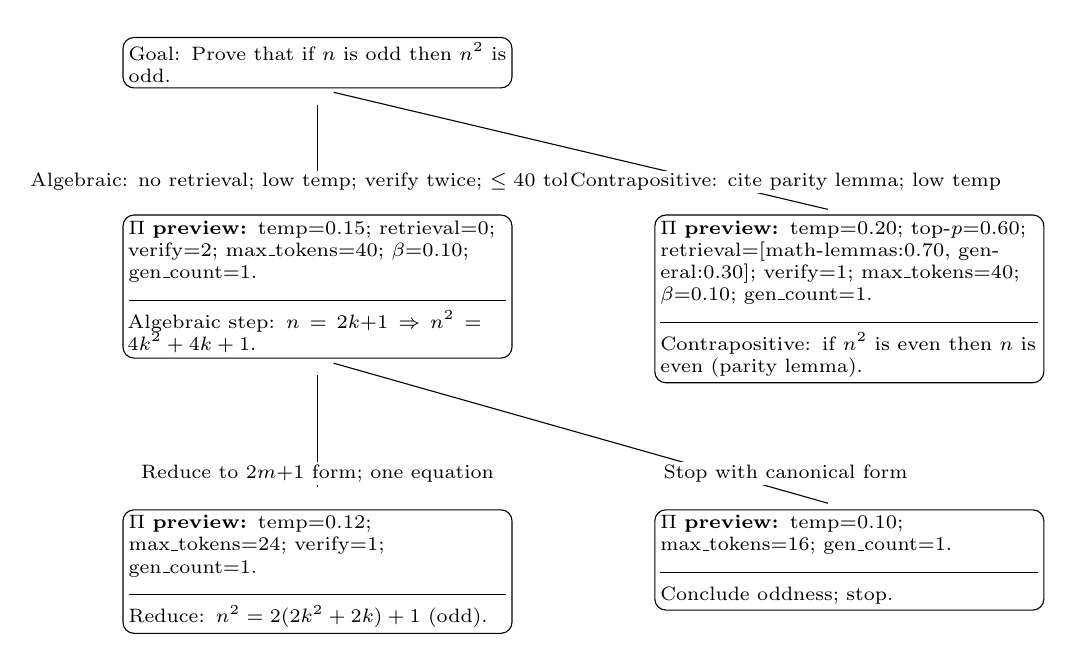
\begin{tikzpicture}[
    node/.style={rectangle, draw, rounded corners, inner sep=2pt, align=left, font=\scriptsize, text width=4.8cm},
    % Two label variants so we can place them above/below and nudge them off the node edge.
    elabelTop/.style={pos=0.88, above, yshift=2pt, fill=white, inner sep=1pt, font=\scriptsize},
    elabelBot/.style={pos=0.88, below, yshift=-2pt, fill=white, inner sep=1pt, font=\scriptsize}
  ]
    %--- Grid with explicit rows: [1, 2, 2] ---
    \matrix[matrix of nodes, row sep=16mm, column sep=18mm] (M) {
      % Row 1 (1 node)
      \node[node] (root) {Goal: Prove that if $n$ is odd then $n^2$ is odd.}; \\
      % Row 2 (2 nodes)
      \node[node] (alg) {%
        \textbf{$\mathrm{\Pi}$ preview:} temp=0.15; retrieval=0; verify=2; max\_tokens=40; $\beta$=0.10; gen\_count=1.%
        \par\noindent\rule{\linewidth}{0.3pt}\vspace{2pt}\\%
        Algebraic step: $n=2k{+}1 \Rightarrow n^2=4k^2+4k+1$.%
      };
      &
      \node[node] (contra) {%
        \textbf{$\mathrm{\Pi}$ preview:} temp=0.20; top-$p$=0.60; retrieval=[math-lemmas:0.70, general:0.30]; verify=1; max\_tokens=40; $\beta$=0.10; gen\_count=1.%
        \par\noindent\rule{\linewidth}{0.3pt}\vspace{2pt}\\%
        Contrapositive: if $n^2$ is even then $n$ is even (parity lemma).%
      }; \\
      % Row 3 (2 nodes; both under the SAME parent 'alg')
      \node[node] (alg_reduce) {%
        \textbf{$\mathrm{\Pi}$ preview:} temp=0.12; max\_tokens=24; verify=1; gen\_count=1.%
        \par\noindent\rule{\linewidth}{0.3pt}\vspace{2pt}\\%
        Reduce: $n^2=2(2k^2+2k)+1$ (odd).%
      };
      &
      \node[node] (alg_stop) {%
        \textbf{$\mathrm{\Pi}$ preview:} temp=0.10; max\_tokens=16; gen\_count=1.%
        \par\noindent\rule{\linewidth}{0.3pt}\vspace{2pt}\\%
        Conclude oddness; stop.%
      }; \\
    };

    %--- Edges (explicit): start at parent.south, end at child.north
    % Shorten near nodes so labels have breathing room and don't overlap the boxes
    \draw[shorten <=6pt, shorten >=8pt] (root.south)
      -- node[elabelTop]{Algebraic: no retrieval; low temp; verify twice; $\leq 40$ tokens}
      (alg.north);

    \draw[shorten <=6pt, shorten >=8pt] (root.south)
      -- node[elabelTop]{Contrapositive: cite parity lemma; low temp}
      (contra.north);

    \draw[shorten <=6pt, shorten >=8pt] (alg.south)
      -- node[elabelTop]{Reduce to $2m{+}1$ form; one equation}
      (alg_reduce.north);

    \draw[shorten <=6pt, shorten >=8pt] (alg.south)
      -- node[elabelTop]{Stop with canonical form}
      (alg_stop.north);
  \end{tikzpicture}
  \caption{A synthetic example of NLEL being used in a ToT setting. For simplicity, gen\_count is set to one for all $\Pi_i$.}
  \label{fig:nlel_schematic}
\end{figure*}
 -----------------------------------------------------------------------

\subsection{Prompt-Only JSON Parameter Emitter (JPE)}
\label{subsec:jpe}
The tuner LM receives three ingredients in the prompt: (i) a concise \emph{schema} that specifies control fields and bounds; (ii) a \emph{historical ledger} of $(P_i,L_i,C_i)\!\mapsto\!\Pi_i$ with outcomes, where rows are tagged as \emph{Pareto} or \emph{dominated} to provide contrastive signals about efficient trade-offs; and (iii) the \emph{current case} $(P,L,C)$. It emits a single JSON object $\Pi$ that must validate against the schema. The ledger can be curated with a lightweight objective that balances task success against compute usage and verification reliability (e.g., success@compute with penalties for excessive tokens or failed checks).

\subsection{Context Features}
To keep $C$ compact and measurable, we surface a small set of features that capture the state of search:
\begin{itemize}
  \item \textbf{Frontier uncertainty:} median $\sigma$ across candidate downstream values (from ensembles, bootstraps, or dropout estimates);
  \item \textbf{Novelty:} median nearest-neighbor distance among frontier candidates (embedding or lexical);
  \item \textbf{Depth:} distance from root (enables exploration annealing and quota schedules);
  \item \textbf{Sibling/frontier summaries:} best $(\mu,\sigma)$ among siblings; raw label history (strings); budget usage.
\end{itemize}

\subsection{Downstream Selection (Agnostic to NLEL)}
We inherit the standard ToT child-selection operator and apply it once to the union of all candidates produced for a parent (across labels).
\subsection{Stability and Safety}
We employ non-intrusive guards: (i) strict schema/bounds validation for emitted JSON; (ii) projection into a trust region around safe defaults to prevent pathological jumps; and (iii) depth-annealed exploration so late-depth expansions remain conservative.

\subsection{Design Notes}
NLEL is compatible with a non-reasoning tuner or a reasoning tuner (e.g., CoT/ToT) used \emph{only} as a controller. The child reasoner can be held fixed to cleanly attribute outcomes to the edge label and the control vector~$\Pi$.

\section{Theory (Optional)}

\section{Experiments}
% TODO: Empirical check for depth annealing (Section 3.7(iii)):
%       Compare depth-annealed exploration vs. no annealing under identical budgets.
%       Measure success@compute and reliability under verification constraints.
% TODO: Ablations on: (a) label vocabularies, (b) tuner type, (c) ledger size.

\section{Limitations}

\section{Conclusion}

\section*{Impact Statement}

% \section*{Acknowledgements}

\bibliographystyle{icml2025}
\bibliography{icml_submission}

\appendix

\section{Additional Experimental Details}
\section{Proofs}
\section{Extra Results}

\end{document}
